%*******************************************************************************
%****************************** Appendix D *************************************
%*******************************************************************************
\chapter{Experiment Design} \label{appendix:d}

%% **************************** Define Graphics Path **************************
\graphicspath{
	{appendixD/experiment_check_list/PDF/}
	{appendixD/participation_sheet/}}



\section{Experiment Check List} \label{appendix:d:ecl}
Figure \ref{fig:ecl} shows the experiment check list for the experiments 
which consist of: 1. Participant Information, 2. Setting up sensors, 
3. Experiments, 4. Stop sensors, and 5. Extra notes.
%%---------------------------------(FIGURE)-------------------------------------
\begin{figure}
 \centering
   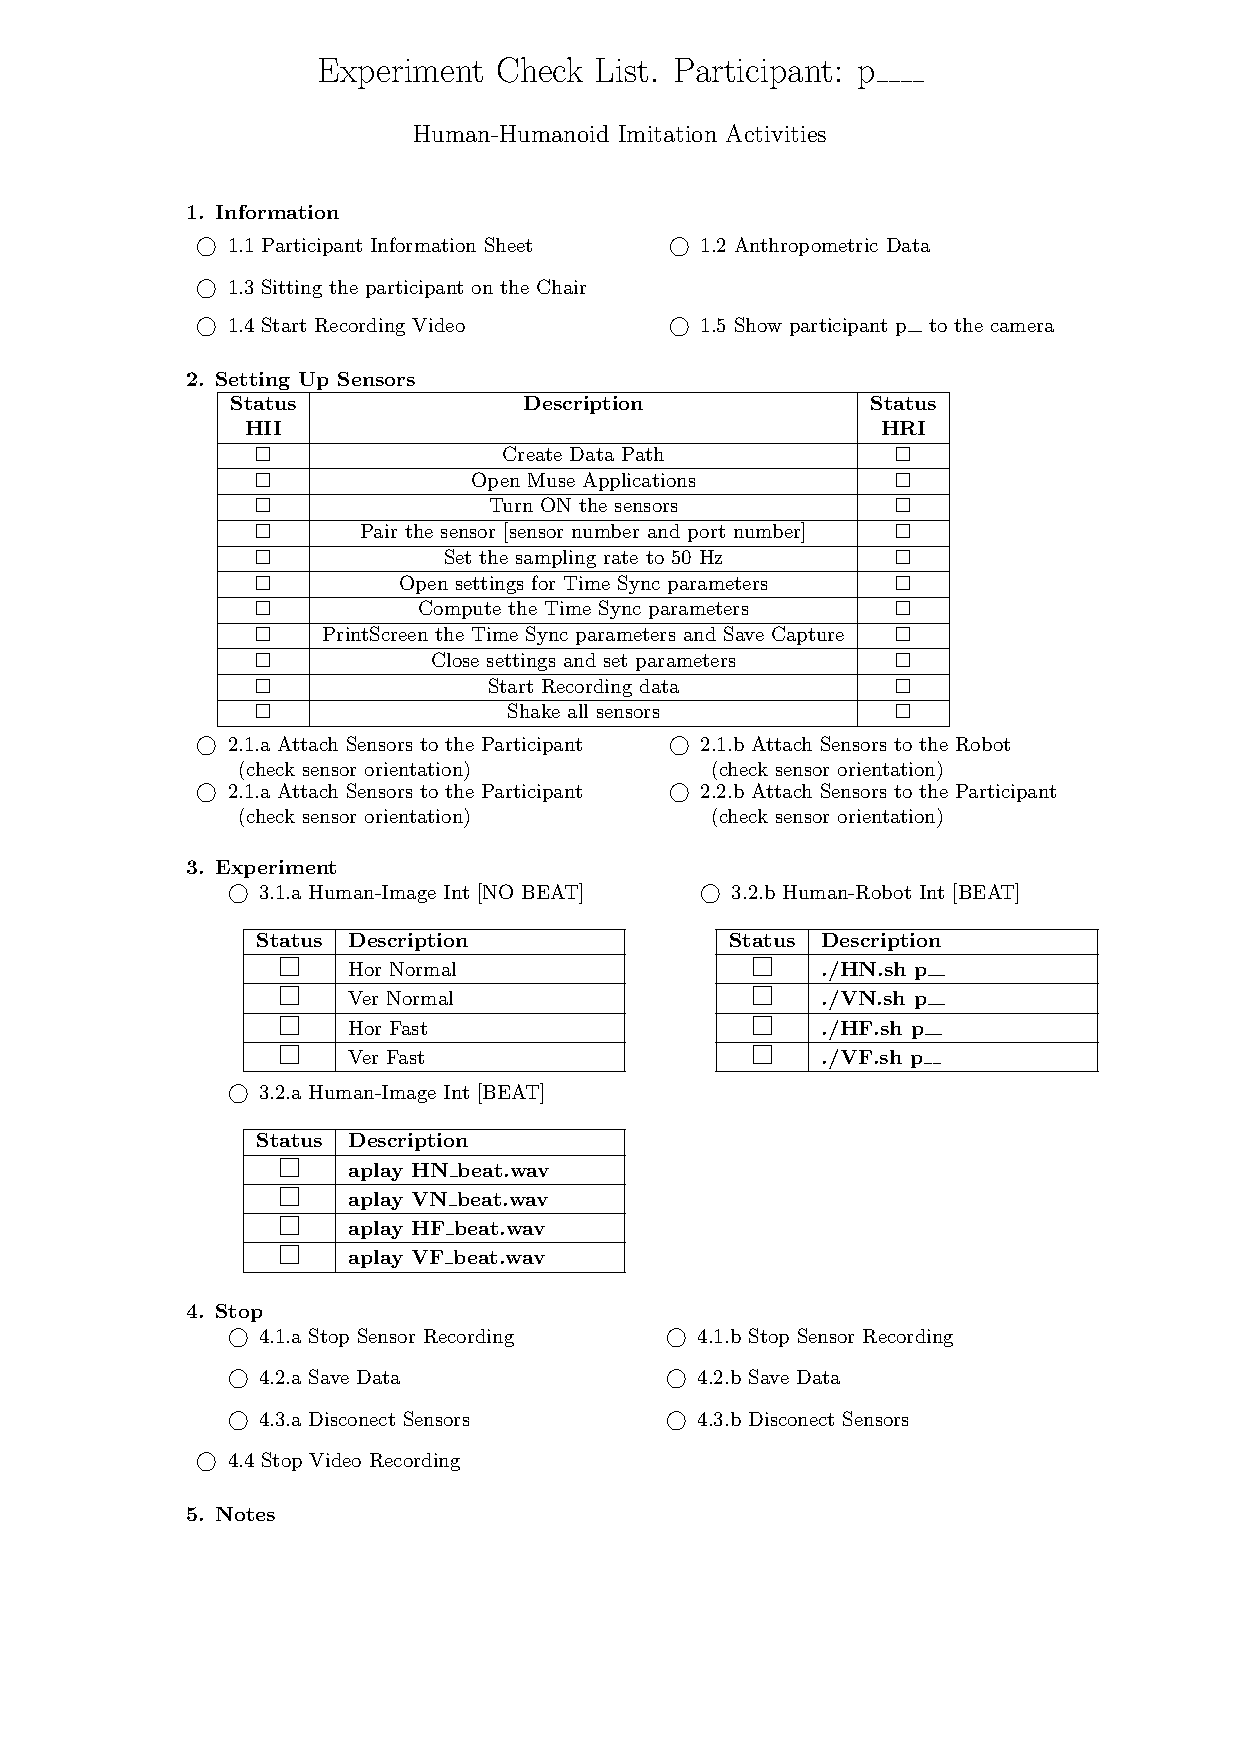
\includegraphics[width=0.95\textwidth]{cl}
   \caption
	[Experiment Check List]{
	{\bf Experiment Check List.}
}
   \label{fig:ecl}
\end{figure}
%%---------------------------------(FIGURE)-------------------------------------


%\newpage
\section{Information Sheet} \label{appendix:d:is}
Figures \ref{fig:epi1}, \ref{fig:epi2}, \ref{fig:epi3} and \ref{fig:epi4}
show a google form for the Online Participation Sheet.

%%---------------------------------(FIGURE)-------------------------------------
\begin{figure}
 \centering
   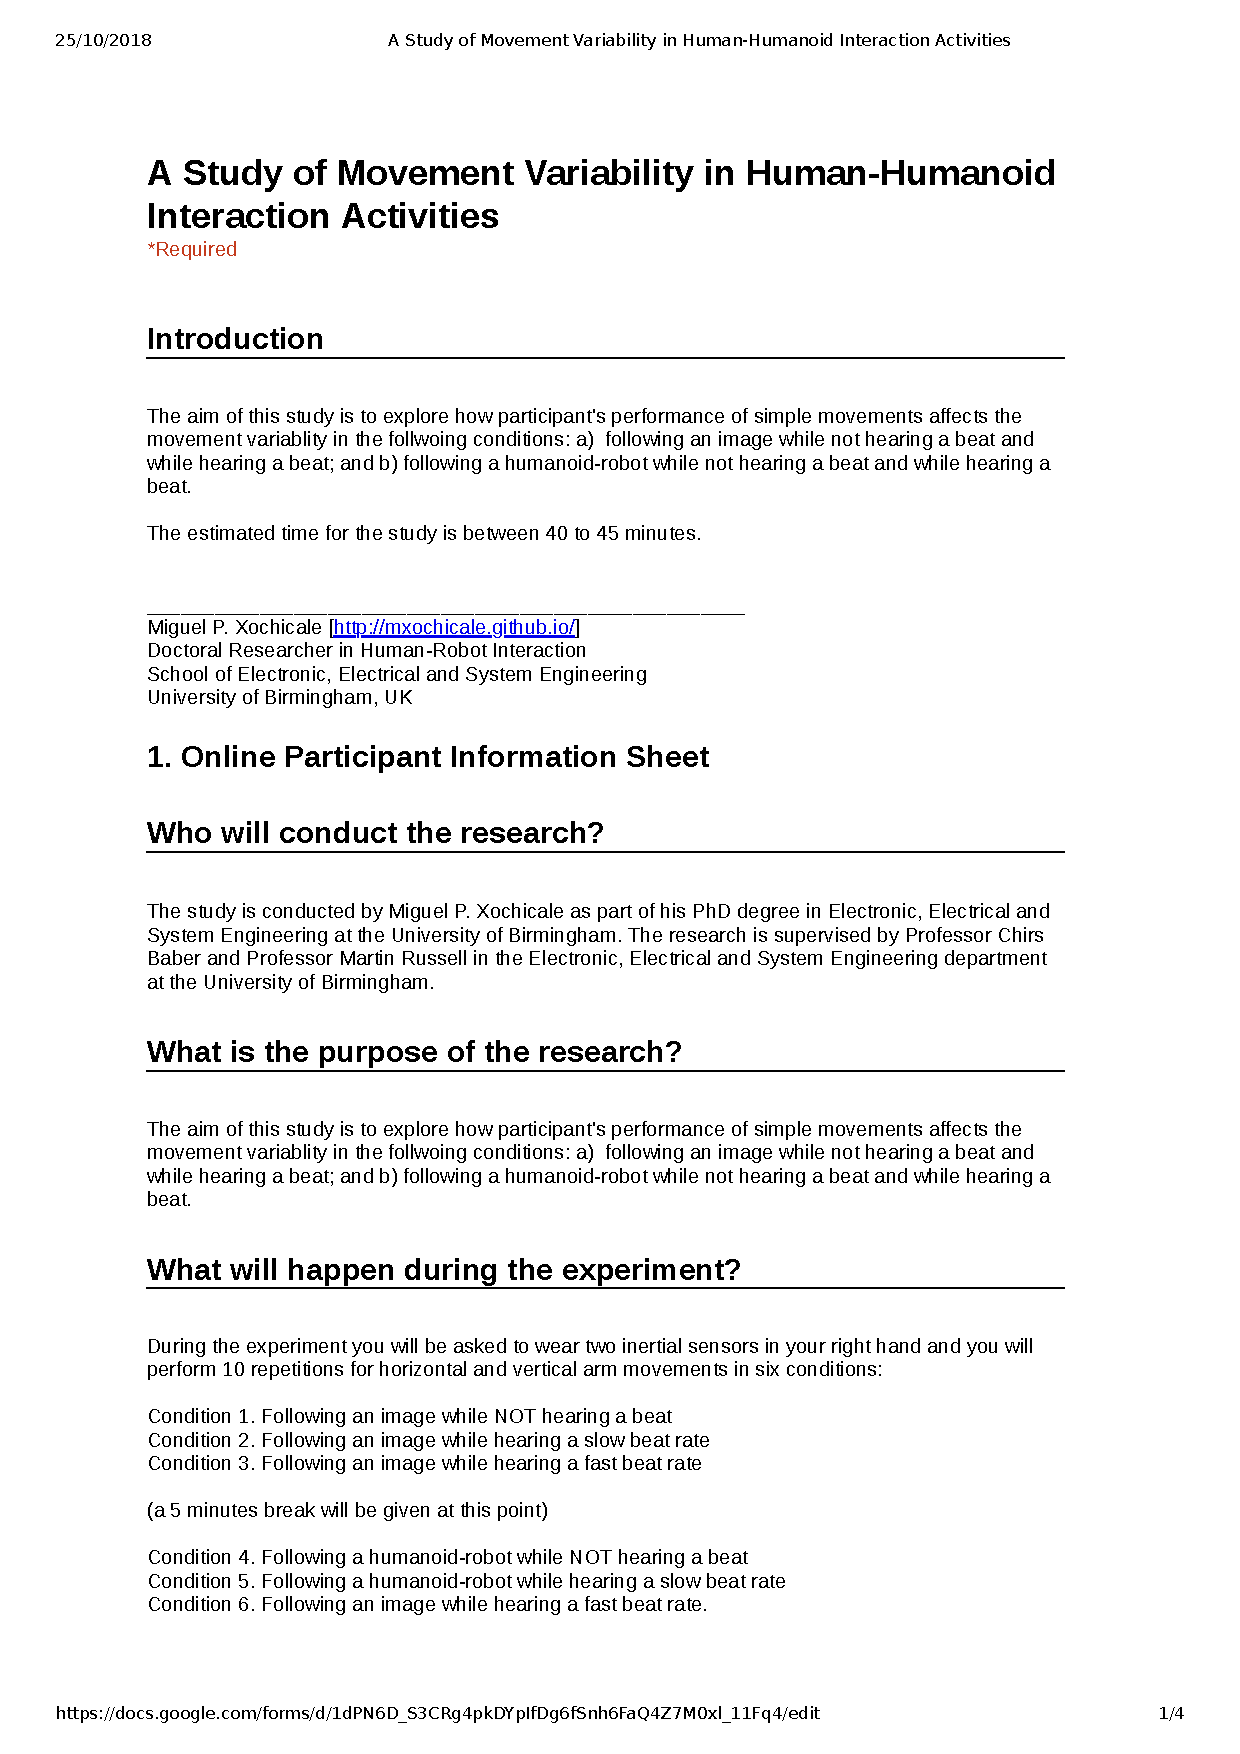
\includegraphics[width=0.9\textwidth]{epi1}
   \caption
	[Participant Information Sheet (p. 1/4) ]{
	{\bf Participant Information Sheet (p. 1/4)}
}
   \label{fig:epi1}
\end{figure}
%%---------------------------------(FIGURE)-------------------------------------
%%---------------------------------(FIGURE)-------------------------------------
\begin{figure}
 \centering
   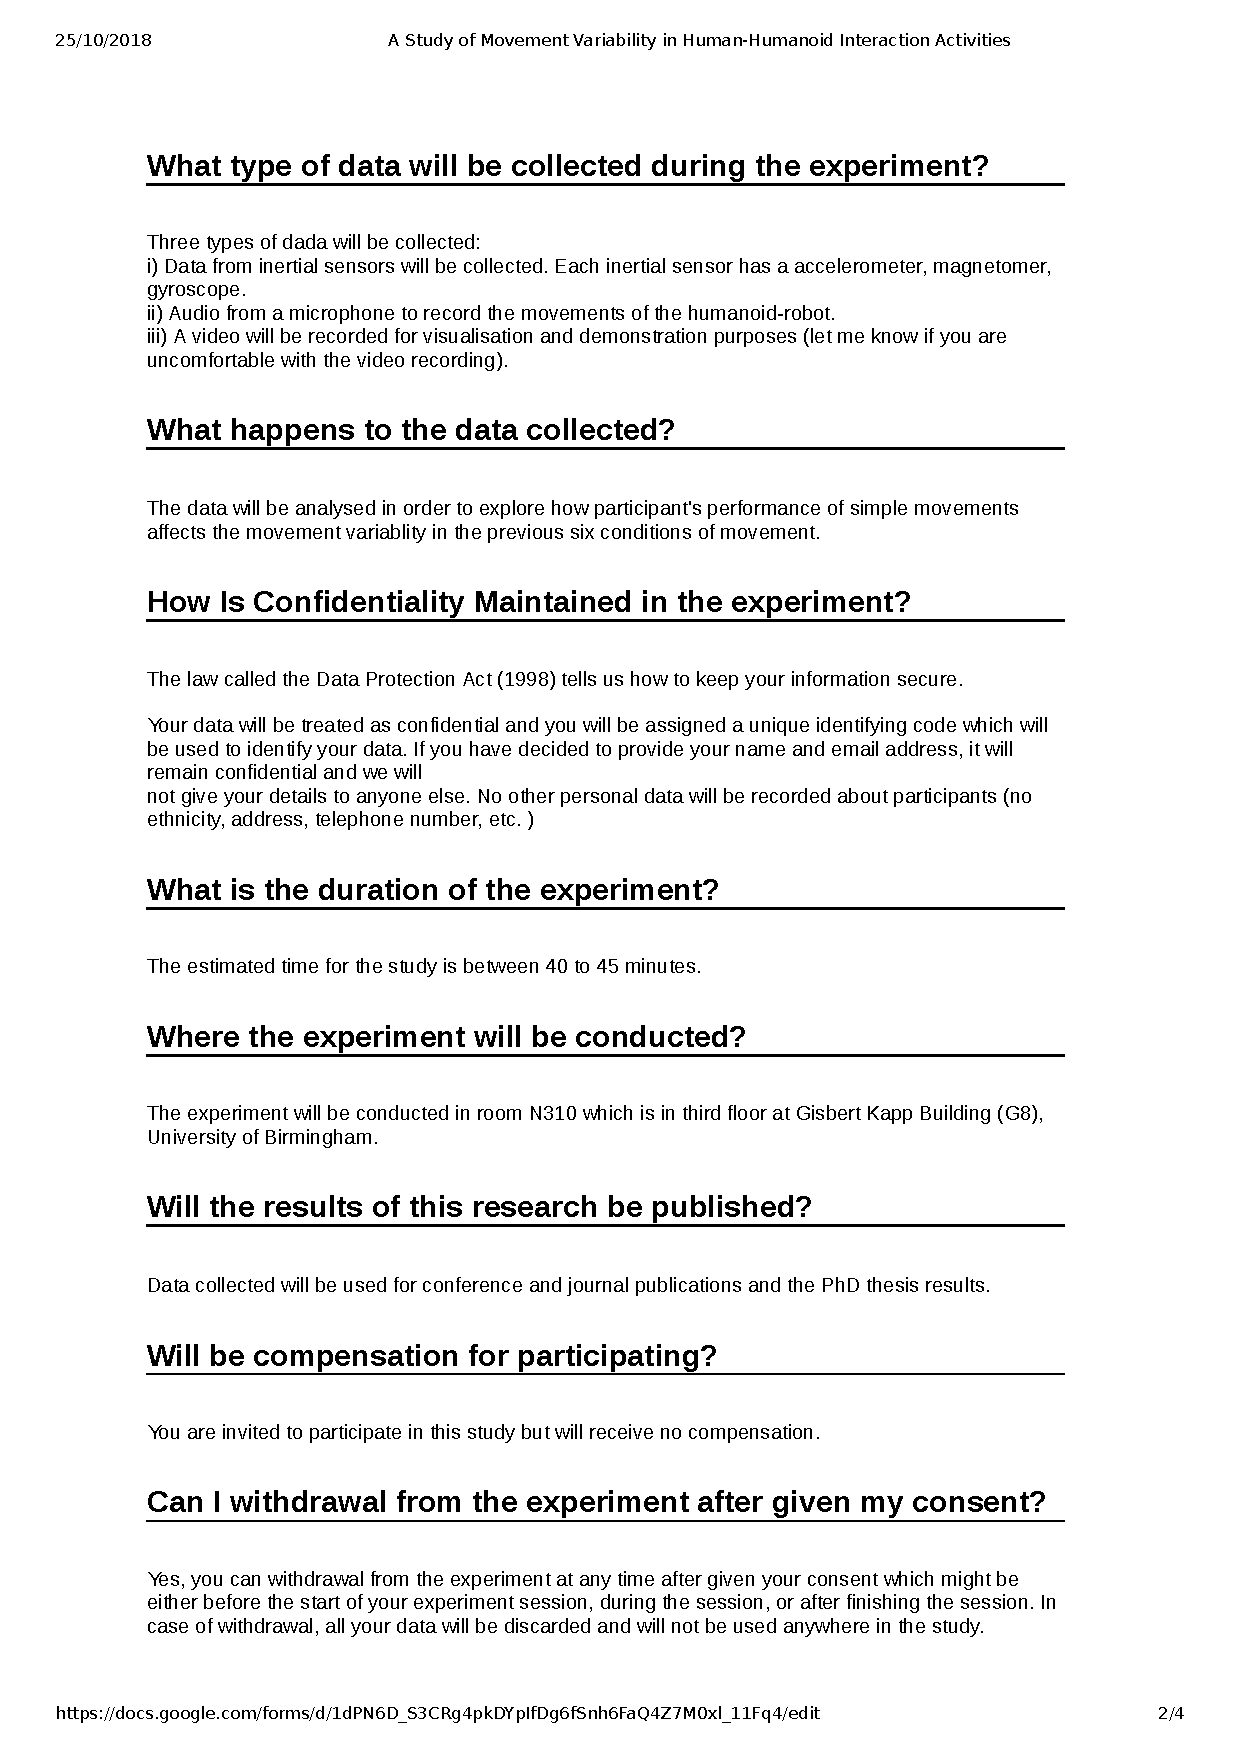
\includegraphics[width=0.9\textwidth]{epi2}
   \caption
	[Participant Information Sheet (p. 2/4) ]{
	{\bf Participant Information Sheet (p. 2/4)}
}
   \label{fig:epi2}
\end{figure}
%%---------------------------------(FIGURE)-------------------------------------
%%---------------------------------(FIGURE)-------------------------------------
\begin{figure}
 \centering
   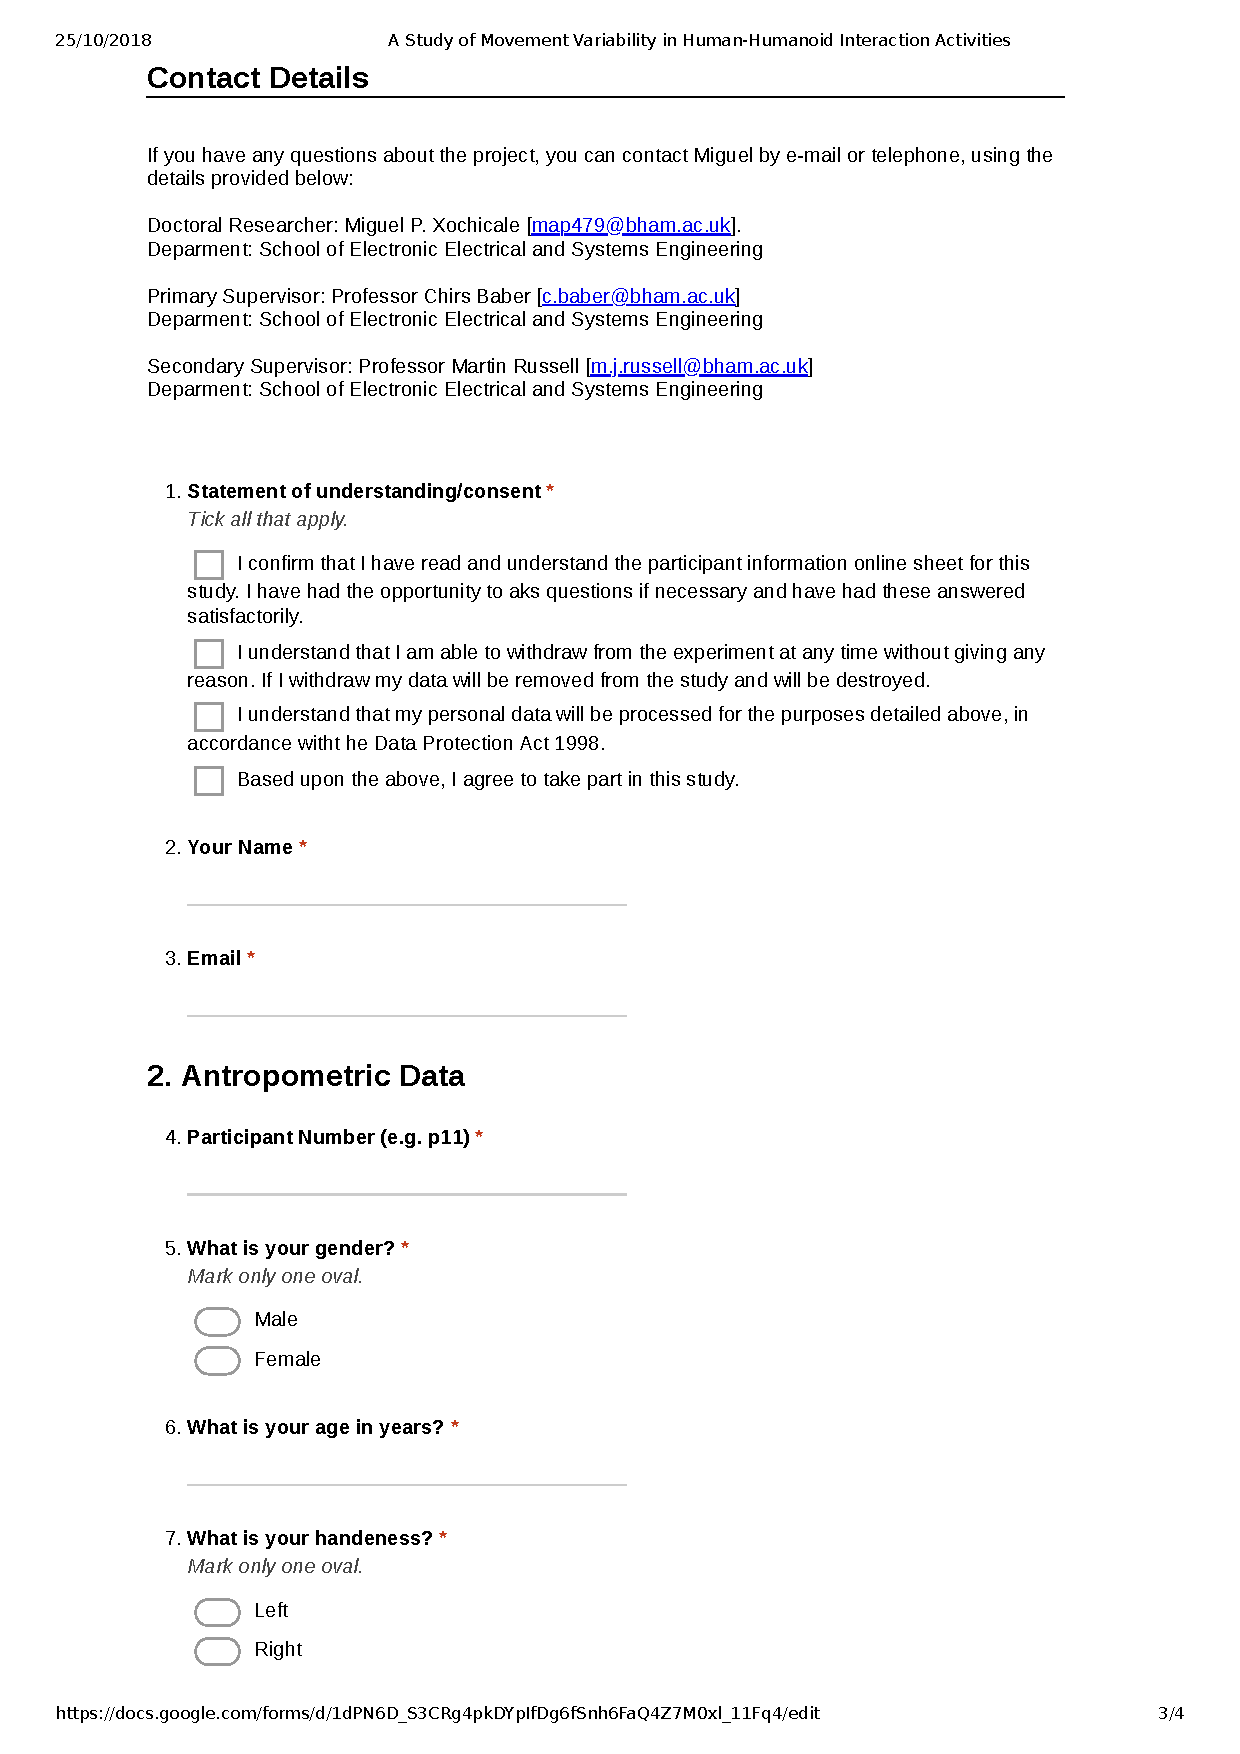
\includegraphics[width=0.9\textwidth]{epi3}
   \caption
	[Participant Information Sheet (p. 3/4) ]{
	{\bf Participant Information Sheet (p. 3/4)}
}
   \label{fig:epi3}
\end{figure}
%%---------------------------------(FIGURE)-------------------------------------
%%---------------------------------(FIGURE)-------------------------------------
\begin{figure}
 \centering
   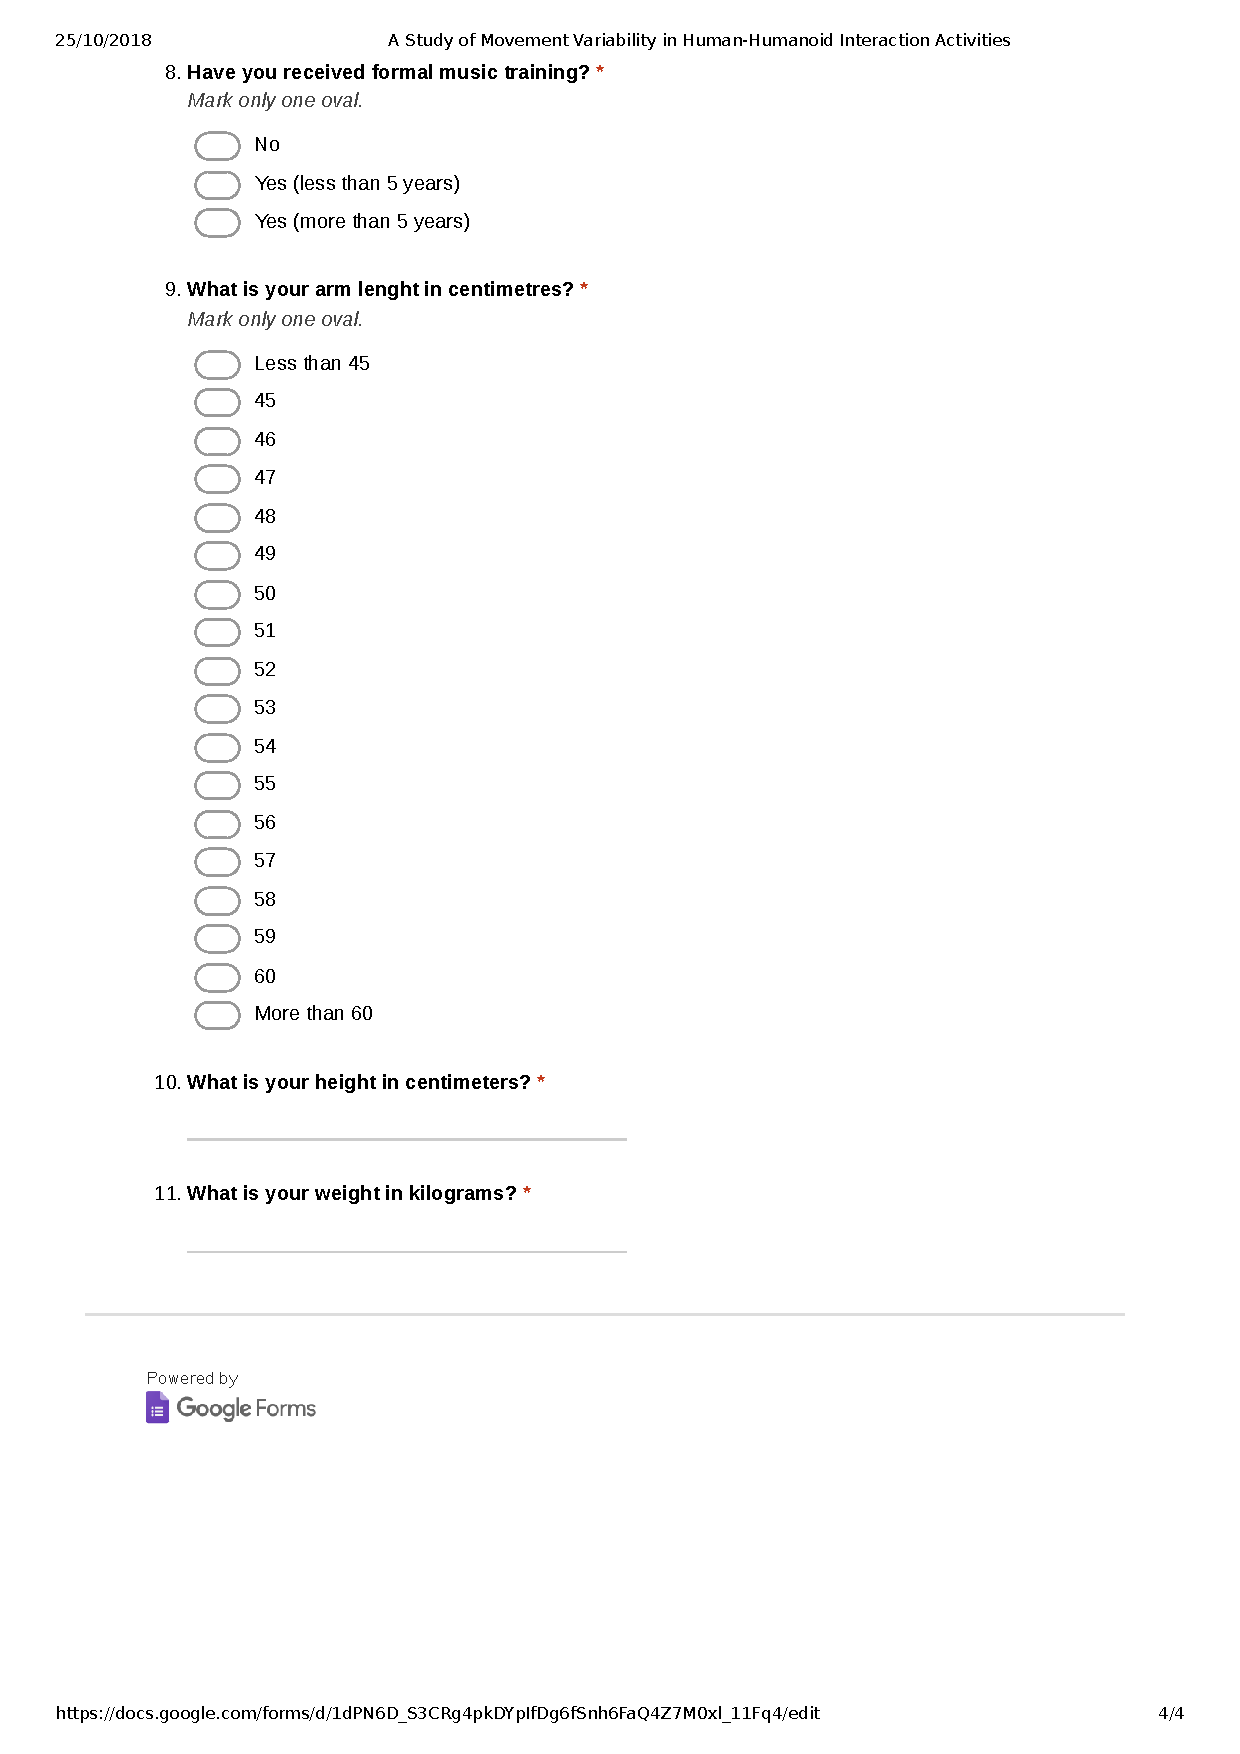
\includegraphics[width=0.9\textwidth]{epi4}
   \caption
	[Participant Information Sheet (p. 4/4) ]{
	{\bf Participant Information Sheet (p. 4/4)}
}
   \label{fig:epi4}
\end{figure}
%%---------------------------------(FIGURE)-------------------------------------



